The measurement of current $I$ was shown in Table \ref{tab-deg-45}.
\begin{table}[!h]
\begin{center}
\begin{tabular}{|c|c|c||c|c|c|}
\hline
\multicolumn{6}{|c|}{Rotation angle of 1/4-wave plate: $45^\circ$}\\
\hline
\multicolumn{6}{|c|}{Maximum Electric Current $I_0$ $2.452\pm0.001$ [$\mu A$]}\\
\hline
$\theta$&$I[\mu A]\pm0.01[\mu A]$&$I/I_0$&$\theta$&$I[\mu A]\pm0.01[\mu A]$&$I/I_0$\\
\hline
$0^\circ$	&	2.350	&	$0.958\pm0.0006$	&	$180^\circ$	&	2.349	&	$0.958\pm0.0006$	\\
\hline
$10^\circ$	&	2.388	&	$0.974\pm0.0006$	&	$190^\circ$	&	2.390	&	$0.975\pm0.0006$	\\
\hline
$20^\circ$	&	2.421	&	$0.987\pm0.0006$	&	$200^\circ$	&	2.431	&	$0.991\pm0.0006$	\\
\hline
$30^\circ$	&	2.441	&	$0.996\pm0.0006$	&	$210^\circ$	&	2.444	&	$0.997\pm0.0006$	\\
\hline
$40^\circ$	&	2.446	&	$0.998\pm0.0006$	&	$220^\circ$	&	2.451	&	$1.000\pm0.0006$	\\
\hline
$50^\circ$	&	2.434	&	$0.993\pm0.0006$	&	$230^\circ$	&	2.441	&	$0.996\pm0.0006$	\\
\hline
$60^\circ$	&	2.410	&	$0.983\pm0.0006$	&	$240^\circ$	&	2.420	&	$0.987\pm0.0006$	\\
\hline
$70^\circ$	&	2.373	&	$0.968\pm0.0006$	&	$250^\circ$	&	2.382	&	$0.971\pm0.0006$	\\
\hline
$80^\circ$	&	2.333	&	$0.951\pm0.0006$	&	$260^\circ$	&	2.333	&	$0.951\pm0.0006$	\\
\hline
$90^\circ$	&	2.297	&	$0.937\pm0.0006$	&	$270^\circ$	&	2.295	&	$0.936\pm0.0006$	\\
\hline
$100^\circ$	&	2.255	&	$0.920\pm0.0006$	&	$280^\circ$	&	2.251	&	$0.918\pm0.0006$	\\
\hline
$110^\circ$	&	2.224	&	$0.907\pm0.0006$	&	$290^\circ$	&	2.222	&	$0.906\pm0.0006$	\\
\hline
$120^\circ$	&	2.211	&	$0.902\pm0.0005$	&	$300^\circ$	&	2.199	&	$0.897\pm0.0005$	\\
\hline
$130^\circ$	&	2.206	&	$0.900\pm0.0005$	&	$310^\circ$	&	2.192	&	$0.894\pm0.0005$	\\
\hline
$140^\circ$	&	2.214	&	$0.903\pm0.0005$	&	$320^\circ$	&	2.204	&	$0.899\pm0.0005$	\\
\hline
$150^\circ$	&	2.237	&	$0.912\pm0.0006$	&	$330^\circ$	&	2.232	&	$0.910\pm0.0006$	\\
\hline
$160^\circ$	&	2.267	&	$0.925\pm0.0006$	&	$340^\circ$	&	2.267	&	$0.925\pm0.0006$	\\
\hline
$170^\circ$	&	2.313	&	$0.943\pm0.0006$	&	$350^\circ$	&	2.303	&	$0.939\pm0.0006$	\\
\hline
\end{tabular}
\caption{Measurement data for the 1/4-wave plate (rotation angle $45^\circ$).}\label{tab-deg-45}
\end{center}
\end{table}

The relation between rotation angle and light intensity was plotted in Figure \ref{fig-deg-45}.
\begin{figure}[H]
\centering
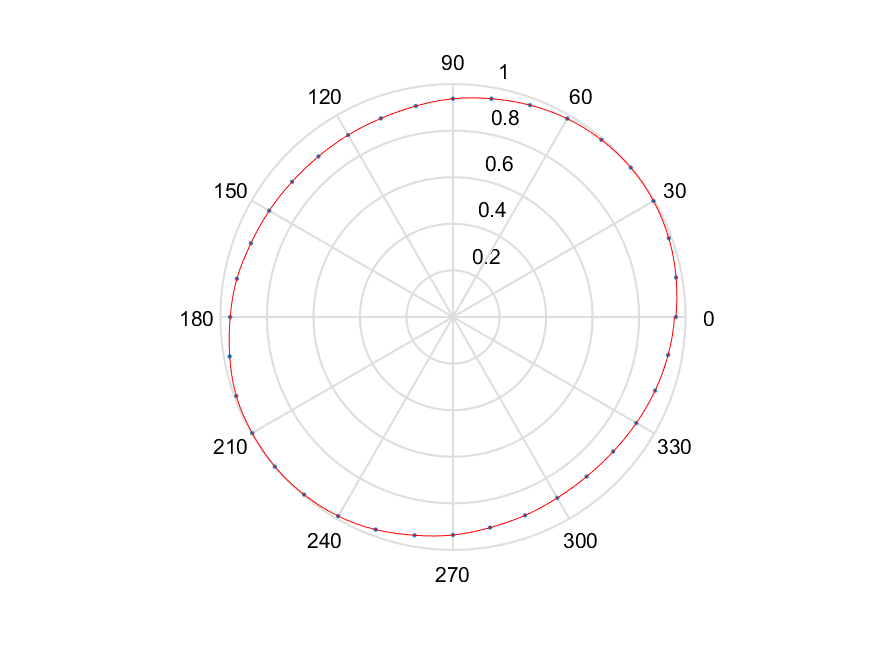
\includegraphics[scale=0.5]{deg-45.png}
\caption{$\theta$ vs. $I/I_0$ graph.}
\label{fig-deg-45}
\end{figure}
